%!TEX root = ../main.tex
\chapter{Reti convoluzionali e varianti non codificanti}\label{chp:CNN-non-coding-variants}

In questo capitolo verranno presentati tre tool basati su reti neurali convoluzionali, sviluppati con l'obiettivo di migliorare la comprensione funzionale delle mutazioni non codificanti. I modelli trattati sono \textsl{DeepSEA}\,\cite{zhou2015predicting}, \textsl{Basset}\,\cite{kelley2016basset} e \textsl{DeepSATA}\,\cite{ma2023deepsata}. Ciascuno di questi modelli verrà approfonditamente analizzato, in modo da comprendere le caratterstiche principali di ciascuno strumento. Più precisamente sarà discusso il dataset utilizzato per allenare il modello, la sua struttura — quindi il numero ed il tipo di livelli presenti — e le tecniche di allenamento applicate.





\section{DeepSEA}\label{sec:DeepSEA}
% 
Il primo tool che verrà analizzato è DeepSEA (\textit{Deep learning-based Saquence Analizer}), introdotto nel 2015 con l'obiettivo di predire l'effetto delle varianti non codifcanti nella cromatina. Al fine di garantire una previsione accurata, questo modello considera lunghe sequenze di \acs{DNA} in modo da conoscere in maniera migliore il contesto in cui avviene la mutazione e quindi comprenderne le funzionalità, anche grazie alla struttura gerarchica dei livelli convoluzionali, che permettono di esaminare pattern locali e globali. 
Inoltre, DeepSEA è in grado di imparare contemporaneamente diverse funzionalità della cromatina utilizzando un approccio di multitask learning, che permette di addestrare il modello su più compiti correlati nello stesso momento. Per comprendere in maniera più approfondita gli effetti funzionali delle mutazioni non codificanti, è stato allenato in modo da predire 919 profili di cromatina suddivisi in tre macro categorie:
% 
\begin{itemize}
    \item 690 tipi di sequenze associate ai siti di binding dei fattori di trascrizone (\acs{TF}), che giocano un ruolo fondamentale durante la trascrizione;
    \item 125 profili di regioni ipersensibili all'enzima DNasi I (\acs{DHS}), che indicano la presenza o meno di elementi regolativi nel \acs{DNA}, anche questi importanti durante la fase di trascrizione;
    \item 104 profili di modifiche istoniche, ovvero mutazioni negli istoni che rendono poco accessibile il \acs{DNA} nella cromatina, impedendo quindi una corretta trascrizione;
\end{itemize}
% 

Il modello — implementato con la libreria \href{https://github.com/torch/torch7}{\textsl{Torch7}} — è composto da esattmente tre livelli convoluzionali: il primo livello contiene 320 filtri, il secondo 480 e l'ultimo contiene 960 kernel. I filtri sono delle \textit{Position Weight Matrix} (\acs{PWM}), ovvero delle matrici composte da $4$ righe ed $M$ colonne che, per ciascuna base azotata, indicano la probabilità che appaia in quella determinata posizione, come mostrato nella Figura\,\ref{fig:PWM}.
% 
\begin{figure}[!b]
    \centering
    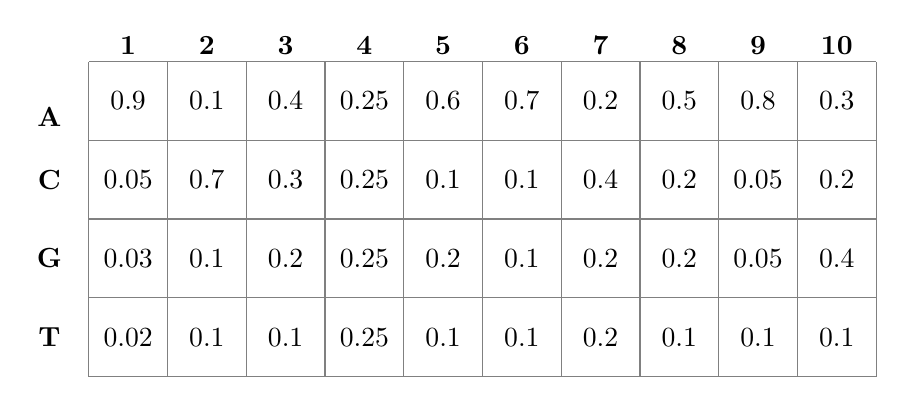
\begin{tikzpicture}
    \node at (-0.5,3.3) {\textbf{A}};
    \node at (-0.5,2.5) {\textbf{C}};
    \node at (-0.5,1.5) {\textbf{G}};
    \node at (-0.5,0.5) {\textbf{T}};
    
    \draw[step=1cm,gray,thin] (0,0) grid (10,4); % Grid 10x4

    \node at (0.5,3.5) {0.9}; \node at (0.5,2.5) {0.05}; \node at (0.5,1.5) {0.03}; \node at (0.5,0.5) {0.02};
    \node at (1.5,3.5) {0.1}; \node at (1.5,2.5) {0.7};  \node at (1.5,1.5) {0.1};  \node at (1.5,0.5) {0.1};
    \node at (2.5,3.5) {0.4}; \node at (2.5,2.5) {0.3};  \node at (2.5,1.5) {0.2};  \node at (2.5,0.5) {0.1};
    \node at (3.5,3.5) {0.25}; \node at (3.5,2.5) {0.25}; \node at (3.5,1.5) {0.25}; \node at (3.5,0.5) {0.25};
    \node at (4.5,3.5) {0.6}; \node at (4.5,2.5) {0.1};  \node at (4.5,1.5) {0.2};  \node at (4.5,0.5) {0.1};
    \node at (5.5,3.5) {0.7}; \node at (5.5,2.5) {0.1};  \node at (5.5,1.5) {0.1};  \node at (5.5,0.5) {0.1};
    \node at (6.5,3.5) {0.2}; \node at (6.5,2.5) {0.4};  \node at (6.5,1.5) {0.2};  \node at (6.5,0.5) {0.2};
    \node at (7.5,3.5) {0.5}; \node at (7.5,2.5) {0.2};  \node at (7.5,1.5) {0.2};  \node at (7.5,0.5) {0.1};
    \node at (8.5,3.5) {0.8}; \node at (8.5,2.5) {0.05}; \node at (8.5,1.5) {0.05}; \node at (8.5,0.5) {0.1};
    \node at (9.5,3.5) {0.3}; \node at (9.5,2.5) {0.2};  \node at (9.5,1.5) {0.4};  \node at (9.5,0.5) {0.1};

    \foreach \x in {1,...,10} {
        \node at (\x-0.5, 4.2) {\textbf{\x}};
    }
\end{tikzpicture}

    \caption[Rappresentazione di una \acs{PWM}.]{Rappresentazione di una \acs{PWM} che viene utilizzata come filtro all'interno di una \acs{CNN}.}\label{fig:PWM}
\end{figure}
% 
I filtri analizzano la sequenza in input e, attraverso la convoluzione, estraggono pattern significativi, man mano spostando la finestra di una base della sequenza. Nel primo livello il kernel ha dimesnione $M\times 4$, dove $M$ è la lunghezza della finestra mentre $4$ sono il numero delle basi azotate. I livelli convoluzionali successivi hanno invece dimensione $M\times k$, dove in questo caso $k$ è il numero di kernel che sono stati utilizzati nel livello convoluzionale precedente. Dopo ogni livello convoluzionale viene applicata una \acs{ReLU} (Figura\,\ref{fig:relu-function}) e poi viene inserito un max-pooling layer, volto ad estrarre la feature predominante dal risultato della convoluzione. In questo caso la finestra di pooling non ha uno step di uno, bensì lo step coincide con la lunghezza della finestra stessa. Infine, dopo i tre livelli convoluzionali, è presente un fully connected layer — che riceve il risultato del max-pooling layer della terza convoluzione e ci applica una \acs{ReLU} — e l'output layer, che processa le informazioni con una funzione sigmoide (Figura\,\ref{fig:sigmoid-function}) la quale calcola la probabilità che la sequenza in input corrisponda o meno a una tra i 919 profili.

I 919 profili di cromatina sono stati ottenuti dai progetti ``\textit{Encyclopedia of \acs{DNA} Elements}'' (\acs{ENCODE}) e ``\textit{Roadmap Epigenomics}''. Le sequenze estratte sono state divise in frammenti (\textit{bin}) da 200\,bp\footnote{Con ``\,bp'', si intende \textit{base pair}, ovvero la lunghezza della sequenza espressa nel numero di coppie di basi.}, per un totale di $521\,636\,200$\,bp. Ciascuno di questi bin è stato poi etichettato ad uno tra i 919 profili di cromatina se almeno più della metà della sequenza corrispondeva al profilo teorico. Ogni bin estratto è stato centrato su una sequenza di 1000\,bp di genoma umano, al fine di fornire a DeepSEA maggiore contesto per ricavare informazioni più significative. Ciascuna sequenza di input è stata trasformata in una matrice $1000\times 4$ attraverso il \textit{One-Hot encoding} che trasforma la sequenza unidimensionale in una matrice bidimensionale. Più precisamente le basi azotate, attraverso il One-Hot encoding, sono codificate come segue: $A \to \left[1, 0, 0, 0\right]$, $T \to \left[0, 1, 0, 0\right]$, $C \to \left[0, 0, 1, 0\right]$ e $G \to \left[0, 0, 0, 1\right]$. Infine alla matrice viene associata al rispettivo vettore di \textit{label} che contiene la risposta attesa dalla rete.

Per allenare DeepSEA in maniera efficace si è definita la cost function come la \textit{Negative Log Likelihood} (\acs{NLL}) — chiamata anche \textit{Binary Cross Entropy} (\acs{BCE}) — definita come segue:
% 
\begin{gather*}
    \mathbf{NLL} = - \sum_s \sum_p\, \log\left[ y_{s,\,p}\,\sigma_p\left(X_s\right)  + \left( 1- y_{s,\,p} \right)\left(1 - \sigma_p\left(X_s\right) \right) \right]
\end{gather*}
% 
\noindent In questa formula, $s$ è l'indice del campione $s$-esimo ($X_s$) del dataset e $p$ è l'indice del profilo della cromatina. Ne consegue che il valore $y_{s,\,p}$ è il valore corretto del campione $s$ rispetto al profilo di cromatina $p$ mentre $\sigma_p\left(X_s\right)$ è la predizione di DeepSEA sul campione $X_s$ rispetto al profilo $p$. L'effettiva cost function in realtà è definita come la funzione \acs{NLL} sommata ad altri valori con l'obiettivo di evitare situazioni di \textit{overfitting}\footnote{L'overfitting è la situazione in cui il modello è completamente allineato con il dataset di allenamento, diventando quindi meno accurato nella predizioni di dati che non sono presenti nel datase.}. Il gradiente della loss function è stato calcolato attraverso l'algoritmo della backpropagation, per poi essere utilizzato nell'ottimizzazione della rete. L'algoritmo di ottimizzazione utilizzato è stato il \acs{SGD} con momento, che è una variante utilizzata per aumentare ancora di più le possibilità di non cadere nei minimi locali\,\cite{aggarwal2018neural}. Inoltre si è scelto di applicare il \textit{dropout training} il quale implica di annullare l'effetto di alcuni neuroni durante le epoche dell'allenamento al fine di rendere la rete più robusta al rischio di overfitting\,\cite{nielsen2015neural}.

\begin{comment}
Il modello è stato elaborato per predire l'effetto delle varianti non codificanti sulla cromatina. Sono presenti tre features importanti in questo modello:
\begin{enumerate}
    \item Il modello considera non solo sequenze brevi ma anche lunghe in modo da catturare informazioni più rilevanti contenute su sequenze più ampie, in modo da avere una visione ad insieme delle funzionalità
    \item Il modello riesce a apprendere pattern da diverse scale spaziali, in questo modo è possible analizzare pattern locali e globali grazie ad una struttra gerarchica (penso che sia riferita ai conv layer della CNN)
    \item Addestramento contemporaneo su diversi compiti relativi alla cromatina che condividono caratterstiche predittive. In questo modo è possibile apprendere e prevedere aspetti della cromatina.
\end{enumerate}
% 
L'articolo sottolinea l'importanza di utilizzare un contesto di sequenza più ampio perché la sequenza che circonda la posizione della variante determina le proprietà regolatorie della variante stessa e, di conseguenza, è importante per comprendere gli effetti funzionali delle varianti non codificanti: lunghezza di sequenze fino ad 1k\,bp

È stato poi testato il modello. Il risultato AUC per la predizione di chromatine features, tra cui TF binding sites, è stato di 0.958, superando la performance dello stato dell'arte precedente, gkm-SVM che era di 0.896. Inoltre ha ottenuto ottimi risultati anche per il DHS, con una median AUC di 0.923


\subsection*{Model Design}
Il modello presenta sequenze di conv layer e max pooling layer per estrarre man mano le features in scale spaziali diverse (capisci meglio). Alla fine cè un fully connected che permette di eleborare le informazioni e, attraverso una sgmoide, calcola la probabilità di ciascuno dei chromatine facur feature. I kerne sono le wieght matrixes. L'output di cascun conv layer è processato prima da un RElu. L'operazione di convoulzuone nel primo livello equivale a calcolare le PWM scores in un finestra, con step di 1. Nei livelli convoluzionali successivi, il kernel è una PWM sull'output del layer precedente. 

Nei livelli successivi al primo, il kernel è di dimension MxN, dove N è il numero di kernel utilizzati nel layer precedente. Se nel primo livello sono state utilizzate 10 PWM $12\times4$, nel lvl successivo sarà usata un kernel di dimension 12X10. Dopo il convlayer viene pushato un relu e poi u pooling: step = dimensione della pooling window.

In DeepSEA sono presenti 3 livelli convluzionali, il primo con 320 kernel, il secondo con 480 ed il terzo con 960. DOpo la convoluzione è presente un fully connected layer, dove i neuroni ricevono il risultato delle convoluzioni e fanno una relu con la matrice dei pesi che colelga 3conv-FCL (fylly conn layer)

The last layer, the sigmoid output layer, makes predictions for each of the 919 chromatin features (125 DNase features, 690 TF features, 104 histone features) and scales predictions to the 0 to 1 range by the sigmoid function

\subsection*{Model Training}
Si è definita la funzione obiettivo (cost function) come la somma del logaritmo negativo della likelihood (NLL), sommati ad altri parametri per evitare overfitting.
% 

% 
% Dove $s$ indica l'indece del sample e $f$ indica la sua feature (ovvero i vari tipo di output, che sono 919). Inoltre $y_f_s$ indica il label 0,1 rispetto alla al tipo di cromatine featre $f$ e al sample $s$. Infine $\sigma_f\left(X_s\right)$ indica il valore predetto dalla rete dato il sample $s$ sulla feture $f$.

A questa funzione vengono sommati altri attributi alla NLL al fine di evitare l'verfitting.

% 
\begin{gather*}
C = \mathbf{NLL} + \lambda_1\vert\vert W \vert\vert_2^2 + \lambda_2 \vert\vert H^{-1} \vert\vert_1
\end{gather*}
% 




\subsection*{Training dataset}

% , ottenuti dai progetti ``\textit{Encyclopedia of DNA Elements}'' (\acs{ENCODE}) e ``\textit{Roadmap Epigenomics}'' e

Le labels sono stte ricavate da ENCODE e Roadmap Epigenomica. Splittato il genoma in segmenti da 200\,bp. Per ogi frammento sono state associate le 919 chromatine features. Se più del 50\% del frammento era nella peak region della feature, era labellato a 1, altrimenti zero.

Ogni training sample consisteva nel 1000\,bp sequences, centrata sul frammento (bin) di 200 basi ed associata al vettore di etichette che ontiene le 919 features. In questo modo, le due sequenze di 400 \,bp ai lati davaano più contesto in modo da interpretare meglio il risultato.

% For evaluating performance on the test set, we used area under the receiver operating characteristic curve (AUC). The predicted probability for each sequence was computed as the average of the probability predictions for the forward and complementary sequence pairs.
\end{comment}






\section{Basset}\label{sec:Basset}
% 
Basset\footnote{Il nome richiama il bassotto, noto per le sue capacità olfattive, in analogia con l'abilità del modello di riconoscere pattern.} è un potente strumento sviluppato nel 2016, progettato per analizzare sequenze di DNA e prevedere l'accessibilità di 164 siti ipersensibili alla DNase I (\acs{DHS}), che indicano la presenza di elementi regolativi. Mediante le \acs{ConvNet}, questo modello è quindi in grado di fornire importanti informazioni rigaurdo la fase di trascrizione da \acs{DNA} ad \acs{RNA} anlizzando questi particolari siti della cromatina. Proprio come DeepSEA, la presenza di più livelli convoluzionali facilita la comprensione degli aspetti funzionali derivanti dalle mutazioni nei \acs{DHS}.

Anche Basset, come DeepSEA, è stato implementato utilizzando la libreria \href{https://github.com/torch/torch7}{\textsl{Torch7}}. Questo tool dà la possibilità di personalizzare il modello a piacimento, indicando il numero per ciascun tipo di livello, il numero di filtri (\acs{PWM}) nei livelli convoluzionali, la loro dimensione, la grandezza delle finestre di pooling, il numero di neuroni nei fully-connected layer e vari iperparametri per la fase di allenamento e di test. Attraverso l'ottimizzazione Bayesiana si sono trovati i layer e gli iperparametri ideali per l'architettura. La struttura è composta da tre livelli convoluzionali: il primo livello contiene 300 filtri di lunghezza 19\,bp, il secondo è composto da 200 kernel di lunghezza 11\,bp e il terzo layer ne contiene 200 di lunghezza 7\,bp. È importante sottolineare che dopo ciascun livello convoluzionale, segue un livello che normalizza l'output della convoluzione (\textit{batch normalization}) seguito da una \acs{ReLU} ed un max-pooling layer. In seguito ai tre livelli convoluzionali sono presenti tre fully connected layer, alternati con due \acs{ReLU} e due dropout layer (con coefficiente di 0.3) che, in maniera molto simile a DeepSEA sono utilizzati per prevenire il rischio di overfitting, annullando il contributo di alcuni neuroni casuali durante l'allenamento. Infine l'output layer, attraverso la funzione sigmoide, calcola la probabilità che l'input appartenga ad uno dei 164 \acs{DHS}.

Dei siti ipersensibili alla DNasi I, 125 sono stati estratti da \acs{ENCODE} e 39 ``\textit{Roadmap Epigenomics}''. I dati estratti sono stati processati e tutti i siti sono stati isolati ed arricchiti fino ad avere un dataset iniziale di compostp da sequenze di 600\,bp, per un totale di $2\,071\,886$\,bp. Ciascuna delle sequenze presenti nel dataset sono state poi associate al vettore di label che indicava a quale dei 164 tipi la sequenza apparteneva. Dei 164 tipi, il $17\%$ dei siti sono stati associati a promoters, il $47\%$ è stato classificato come siti intragenici — ovvero all'interno dei geni — e il restante $36\%$ è stato etichettato come siti intergenici — cioè tra i geni. Infine, prima di essere utilizzati nella rete, i siti sono stati processati mediante il One-Hot encoding, formando quindi sequenze di input di dimensione $600\times 4$. Del dataset totale, $71\,886$ basi sono state utilizzate per la fase di test e altre $70\,000$ per la fase di validazione.

Il modello è stato allenato attraverso il \acs{GD} stocastico, cercando di ottimizzare la funzione \acs{BCE} il cui gradiente è stato calcolato mediante la backpropagation. Per prevenire il rischio di overfitting si è applicata la tecnica dell'\textit{early stopping}, facendo terminare l'allenamento dopo 12 epoche che la \textit{validation loss} rimane invariata. % Dopo l'allenamento e la validazione, il modello è stato testato, ottenendo un valore AUC medio di $0.895$ sui \acs{DHS}.

\begin{comment}
\subsection*{Model Design}
Weight matrixes that learn patterns. Nel livello convluzionale l'algoritmo scans le PWM (ovvero i filtri). Come nella altre CNN, durante l'allenamento i kernel imparano a riconoscere pattern importatni. IN questo modo non è ecessario specioficarliu manualmente.
% Prior work has demonstrated that with a sufficiently large data set, deep neural networks can learn far more expressive and accurate models than other common approaches like random forests or kernel methods
Dopo ogni livello convluzionale viene appliocata una relu (rectifier operation). Dopo di che viene fatto un max pooling. % This operation reduces the dimension of the input to the next layer (and thus the computation required in training).
Successivi livelli convuluzionali fanno la stessa cosa del primo. Per le sequene di DNA, i livelli usccessivi catturano interazioni spaziali con le pWM iniziali. SOno presenti 3 livelli convopluzionali (ciascuno con il recfier e la max pooling) e infine due livelli fully connected. Il livello finale pusha fuori 164 predizioni.

Sono stati utilizzati il test AUC che plotta false positive vs true popsitive graph. Come deepsea, anche basset è stato dimostrato essere piu pro di gkm-SVM

Il primo layer convoluzionale ha 300 filters. Dopo ciascun convlayer viene fatta una relu e poi una maxpool.
    
È stata usata la libreria Torch7 di python per l'implementazione.

Dopo il terzo layer convoluzionale si applica un doppoio layer fully conncted che operano una sigmoid transformation per mandare in output i 164 tipi di cellule. INltre We trained to minimize the binary cross entropy loss function, summed over these 164 outputs. Si è calcolto il gradiente della funzione obiettivo con la backpropagation.

\subsection*{Dataset}

We downloaded DNase-seq peak BED format files for 125 cell types from the ENCODE Project Consortium (2012) and 39 cell types from the Roadmap Epigenomics Consortium (2015).

Hanno fatto anche in questo caso il flanking di 600 \,bp: To merge the peaks into one set, we first extended each one from its midpoint to 600 \,bp
\end{comment}





\section{DeepSATA}\label{sec:DeepSATA}
% 
Pubblicato nel 2023, DeepSATA è il terzo tool basato su una \acs{CNN} che si occupa di identificare le \acs{OCR} — regioni aperte della cromatina — cercando di comprenderne anche la funzione. In particolare DeepSATA si concentra sulle mutazioni non codificanti nei siti di \acs{TF} binding non solo in sequenze genomiche umane, ma anche di altre specie animali quali maiali, galline, bovini e topi.

DeepSATA è un modelo basato su DeepSEA.\@ È quindi composto da tre layer convoluzionali, con rispettivamente da 320, 480 e 960 kernel (anche in questo caso rappresentati da \acs{PWM}). Ogni livello convluzionale è seguito da un layer che applica la funzione \acs{ReLU} e poi un max pooling layer estrae dal risultato le feature predominanti. Dopo ciascun livello convoluzionale è presente anche un dropout layer che, come per Basset, aiuta la rete a prevenire il rischio di overfitting. I primi due livelli di dropout hanno un coefficiente di 0.2 mentre il terzo ha un coeffciente di 0.5. Anche in questo tool, ai tre layer convoluzionali, segue un fully-conected layer che prepara i dati all'output layer che, attraverso la funzione sigmoide, calcola la probabilita secondo il quale l'input fornito appartenga ad una tra le \acs{OCR} disponibili.

A differenza di DeepSEA e Basset, il formato della sequenza in input è tridimensionale anzichè a due dimensioni. In particolare La sequenza in input è di dimensione $M \times 4 \times (N + 1)$, dove $M$ è la lunghezza della sequenza in input e $4$ sono le basi azotate. Infine $N + 1$, ovvero la profondità della matrice tridimensionale indica le affinità specifiche che ha la sequenza di input con gli $N$ fattori di trascrizione. A questo numero si aggiunge 1, che è lo strato della codifica One-Hot della sequenza. In questo modo i \acs{TF} associati alla sequenza di input aiutano a comprendere in maniera migliore gli effetti delle mutazioni nella sequenza. I \acs{TF} sono stati ottenuti dal database \textsl{JASPAR} e, mediante \textsl{FIMO}\footnote{Questo software identifica dei motif conosciuti all'interno della sequenza fornita in input.}, sono stati identificati i motif più diffusi. Di questi, sono stati selezionai i primi $N$ fattori di trascrizione più presenti da inserire nel dataset iniziale. Per motivi legati alle risorse disponibili, gli autori dell'articolo hanno scelto $N=10$ siti di legame dei \acs{TF}. 

Il dataset che contiene sequenze di più specie è stato raccolto rispettivamente dai seguenti database:
\begin{itemize}
    \item Le sequenze relative ai topi sono state ottenute dall'\textit{\acs{NCBI} Sequence Read Archive} (\acs{SRA});
    \item I tratti di genoma unamo sono stati ricavati da \acs{ENCODE};
    \item Le sequenze genomiche dei maili sono state ottenute dal \textit{Gene Expression Omnibus} (\acs{GEO});
    \item Le porzioni di \acs{DNA} relative a bovini e polli sono state scaricate dal sito dell'Università della California (\textsl{UC Davis}), nella sezione \textit{Farm Clusters}.
\end{itemize} 
% 
\noindent Dopo aver raccolto tutti i dati necessari, in maniera del tutto analoga a DeepSEA, sono stati divisi in bin da 200\,bp ed etichettati a seconda della \acs{OCR} che rappresentavano: se più della metà della sequenza aveva una corrispondenza con una \acs{OCR}, veniva impostata l'etichetta ad 1 per quella particolare regione della cromatina, altrimenti 0. In secondo luogo, sono stati centrati con sequenze lunghe 400\,bp per avere sequenze di 1000\,bp come input, chiamate anche \textit{Open Chromatin Bin} (\acs{OCB}). Di conseguenza, ciascun bin di input, una volta effettuato il One-Hot encoding è rappresentato da una matrice di dimensione $1000 \times 4 \times 11$.

Essendo DeepSATA un modello basato su DeepSEA, il modelli è stato allenato attraverso il \acs{GD} stocastico con momento per ottimizzare la funzione di binary cross entropy. In maniera del tutto analoga, il gradiente di questa funzione è stato calcolato mediante l'algoritmo della backpropagation

\begin{comment}

DeepSATA è uno framework user-friendly, progettato per identificare le regioni aprte di cromatina (OCR) lungo l'intero genoma e le functional annotation delle varianti non codificanti (con annotazione funzionale si intende il processo di descrivere la struttura e la funzione di un componente del genoma).

Il modello è composto da 3 layer, con 320, 480 e 960, ciascuno dei quali seguito da una relu, max pooling e dropout. E applicata la sigmoide per per generare gli output, ovvero la probabilita per la cromatina. Vengono citati ancora una volta i 200 bins flankati di 400 a dtesta e sinistra per dare contesto. Ogni sequenza in input era tridimensionale. Ricordiamo che la terza dimensione, N + 1, rappresenta le configurazioni di legame dei fattori di trascrizione (TF). In particolare, il primo strato in questa dimensione è la codifica one-hot della sequenza di DNA stessa, mentre i successivi strati (dallo strato 2 allo strato N + 1) codificano le affinità di legame e le posizioni specifiche di ciascun TF. Questo approccio consente al modello di considerare non solo la composizione della sequenza ma anche come diversi TF interagiscono con essa, fornendo un contesto ricco e complesso per l'analisi della regolazione genica.

I dati relativi alle specie, sono stati presi dai seguenti databasse:
\begin{itemize}
    \item Topi, e NCBI Sequence Read Archive (SRA)
    \item Umani, ENCODE
    \item SPecie dei Maiali deiravta da e Gene Expression Omnibus (GEO)
    \item Bovini e polli sono stati prelevati dal sito del UC-DAVi university, californi, Farm Clusters
\end{itemize} 

Per le sequenze di DNA, deepsata estende la matrice bidimensionale che rappresenta la sequenza genomica dopo il onehot encoding (matrice M X 4) in una matrice tridimensionale che incorpora anche le binding configuration dei TFs che sono importanti per capire il contesto di studio. Questi TFs sono selezionati per arricchire il dna bionding motif con le OCR, regioni aperte di cromatina. In seguito, lungo la terza dimensione della matrice, ciascun layer convoluzionale successivo codifica l'affinità di legame (biding) dimension un fattore di trascrizione specifico. La strategia di codifica consiste nell'utilizzare la matrice di probabilità dei pesi di posizione del fattore di trascrizione (TF) per popolare la matrice nel suo sito di legame previsto.

Il genoma è stato diviso in bin da 200\,bp. Ad ogni bin è stata assegnata l'etichetta 0 o 1 se almeno meta dei 200 \,bp confomavano alla ATAC peak region. Ogni OCB (Open chromatin bins), associato ai sui 400\,bp di flanking sequence è stato poin buttato dentro deppsata. Ogni OCB è composto dalla strattura $1000 \times 4 \times (N + 1)$, dove N sono i TFs che sono stati predictati legare la sequenza. Per determinare N nel training set sono statti collezionait TF binding sites da Jaspar 2022 database e poi è stato usato FIMO 5.4.1 per identificare la presenza dei motivbi. Dopo di che i TF sono stati rankati i primi N TFS per l'allenamento del modello. Nell'articolo viene indicato che si è deciso di inserire N = 10 a causa di resource constraints.

Copo ciascun layer convoluzionale, viene effettuata una ReLu legegrmente modificata: per evitare gli overfitting, i pesi sono stati messi a 0.000001 quando minori di zero. In seguito alla ReLu viene fatta una maxpooling di grandezza 4 X N + 1, per combinare le feature che sono state estratte dai vari OCB types. Infine, dopo la max pooling viene effettuato un droput con rate di 0.2 per evitare overfitting e rendere a rete pi robusta. Per i livelkli convoluzionali seguenti sono stati utilizzati 480 e 960 kernel. I parametri della ReLu activatioon erano gfli stessi del primo layer. Per quanto riguarda la max pooling, ha size $4 \times 1$, per cionsentire il downsampling del dataset e graantire un miglior traingin experince trolp letsgoski. In questo caso il droput rate è stato butatto a 0.2 e 0.5, per prevenire l'overfitting.
\end{comment}
